\begin{frame}[fragile]
\frametitle{Optimierung von $K$}

\begin{itemize}
  \item Eine Kennlinie an das momentane Signal anpassen
\end{itemize}

\begin{align}
	U_{?, \mathrm{meas}} (t) = \sum_{n=1}^N \, \overline{a}_n \left[ U_{in}(t)\right]^n
	\quad
	U_{?, \mathrm{ideal}} (t) = \sum_{n=1}^N \, a_n \left[ U_{in}(t) \right]^n
\end{align}
\begin{itemize}
  \item Oder direkt über die Differenz der Signale
\end{itemize}
\begin{align}
	\Delta U_? (t) = U_{?, \mathrm{meas}} (t) - U_{?, \mathrm{ideal}} (t)
	=
	\sum_{n=1}^N \, \left( \overline{a}_n -  a_n\right) \left[ U_{in}(t) \right]^n
	=
	\sum_{n=1}^N \, \tilde{a}_n \, \left[ U_{in}(t) \right]^n
\end{align}
\end{frame}

\begin{frame}[fragile]
\frametitle{Optimierung von $K$}
\begin{itemize}
	\item Bestimmung der Parameter $\tilde{a}_n$
	\item Vergleichen der Samples ${\Delta U_{?,i} = \Delta U_? (i \cdot \Delta t)}$ mit ${U_{in,i} = U_{in}(i \cdot \Delta t)}$
\end{itemize}

\begin{align}
	\left( 
	\begin{matrix}
	 	U_{in,1} & U_{in,1}^2 & \dots & U_{in,1}^N \\
		U_{in,2} & U_{in,2}^2 & \dots & U_{in,2}^N \\
		\vdots & \vdots & \ddots & \vdots \\
		U_{,M} & U_{in,M}^2 & \dots & U_{in,M}^N \\
	\end{matrix}
	\right)
	\cdot
	\left(
	\begin{matrix}
		\tilde{a}_1 \\
		\tilde{a}_2 \\
		\vdots \\
		\tilde{a}_N \\	 
	\end{matrix}
	\right) = \left( 
	\begin{matrix}
		\Delta U_{?,1} \\
		\Delta U_{?,2} \\
		\vdots \\
		\Delta U_{?,M} \\	 
	\end{matrix}
	\right)
	\label{eq:Uquest.Gleichungssystem}
\end{align}

\begin{itemize}
	\item Lösung des linearen Optimierungsproblems ergibt die Anpassung der alten Parameter
\end{itemize}
\begin{align}
	a_n^{i+1} = a_n^{i} + \sigma_{a}^{i} \tilde{a}_n^{i}
\end{align}
\end{frame}

%\begin{frame}
%\frametitle{Erster Ansatz}
%\begin{itemize}
%	\item $K$ im gleichen Spannungsbereich anpassen
%	\item Referenz zum Rechnen $U_{out,ideal}$ mit $V_{PP}=\SI{6}{\V}$
%	\item Eingangsspannung mit $V_{PP}=\SI{587}{\mV}$
%\end{itemize}
%\end{frame}

\begin{frame}
\frametitle{Erster Ansatz}
\begin{picture}(10,7)
		\put(0,-160){
			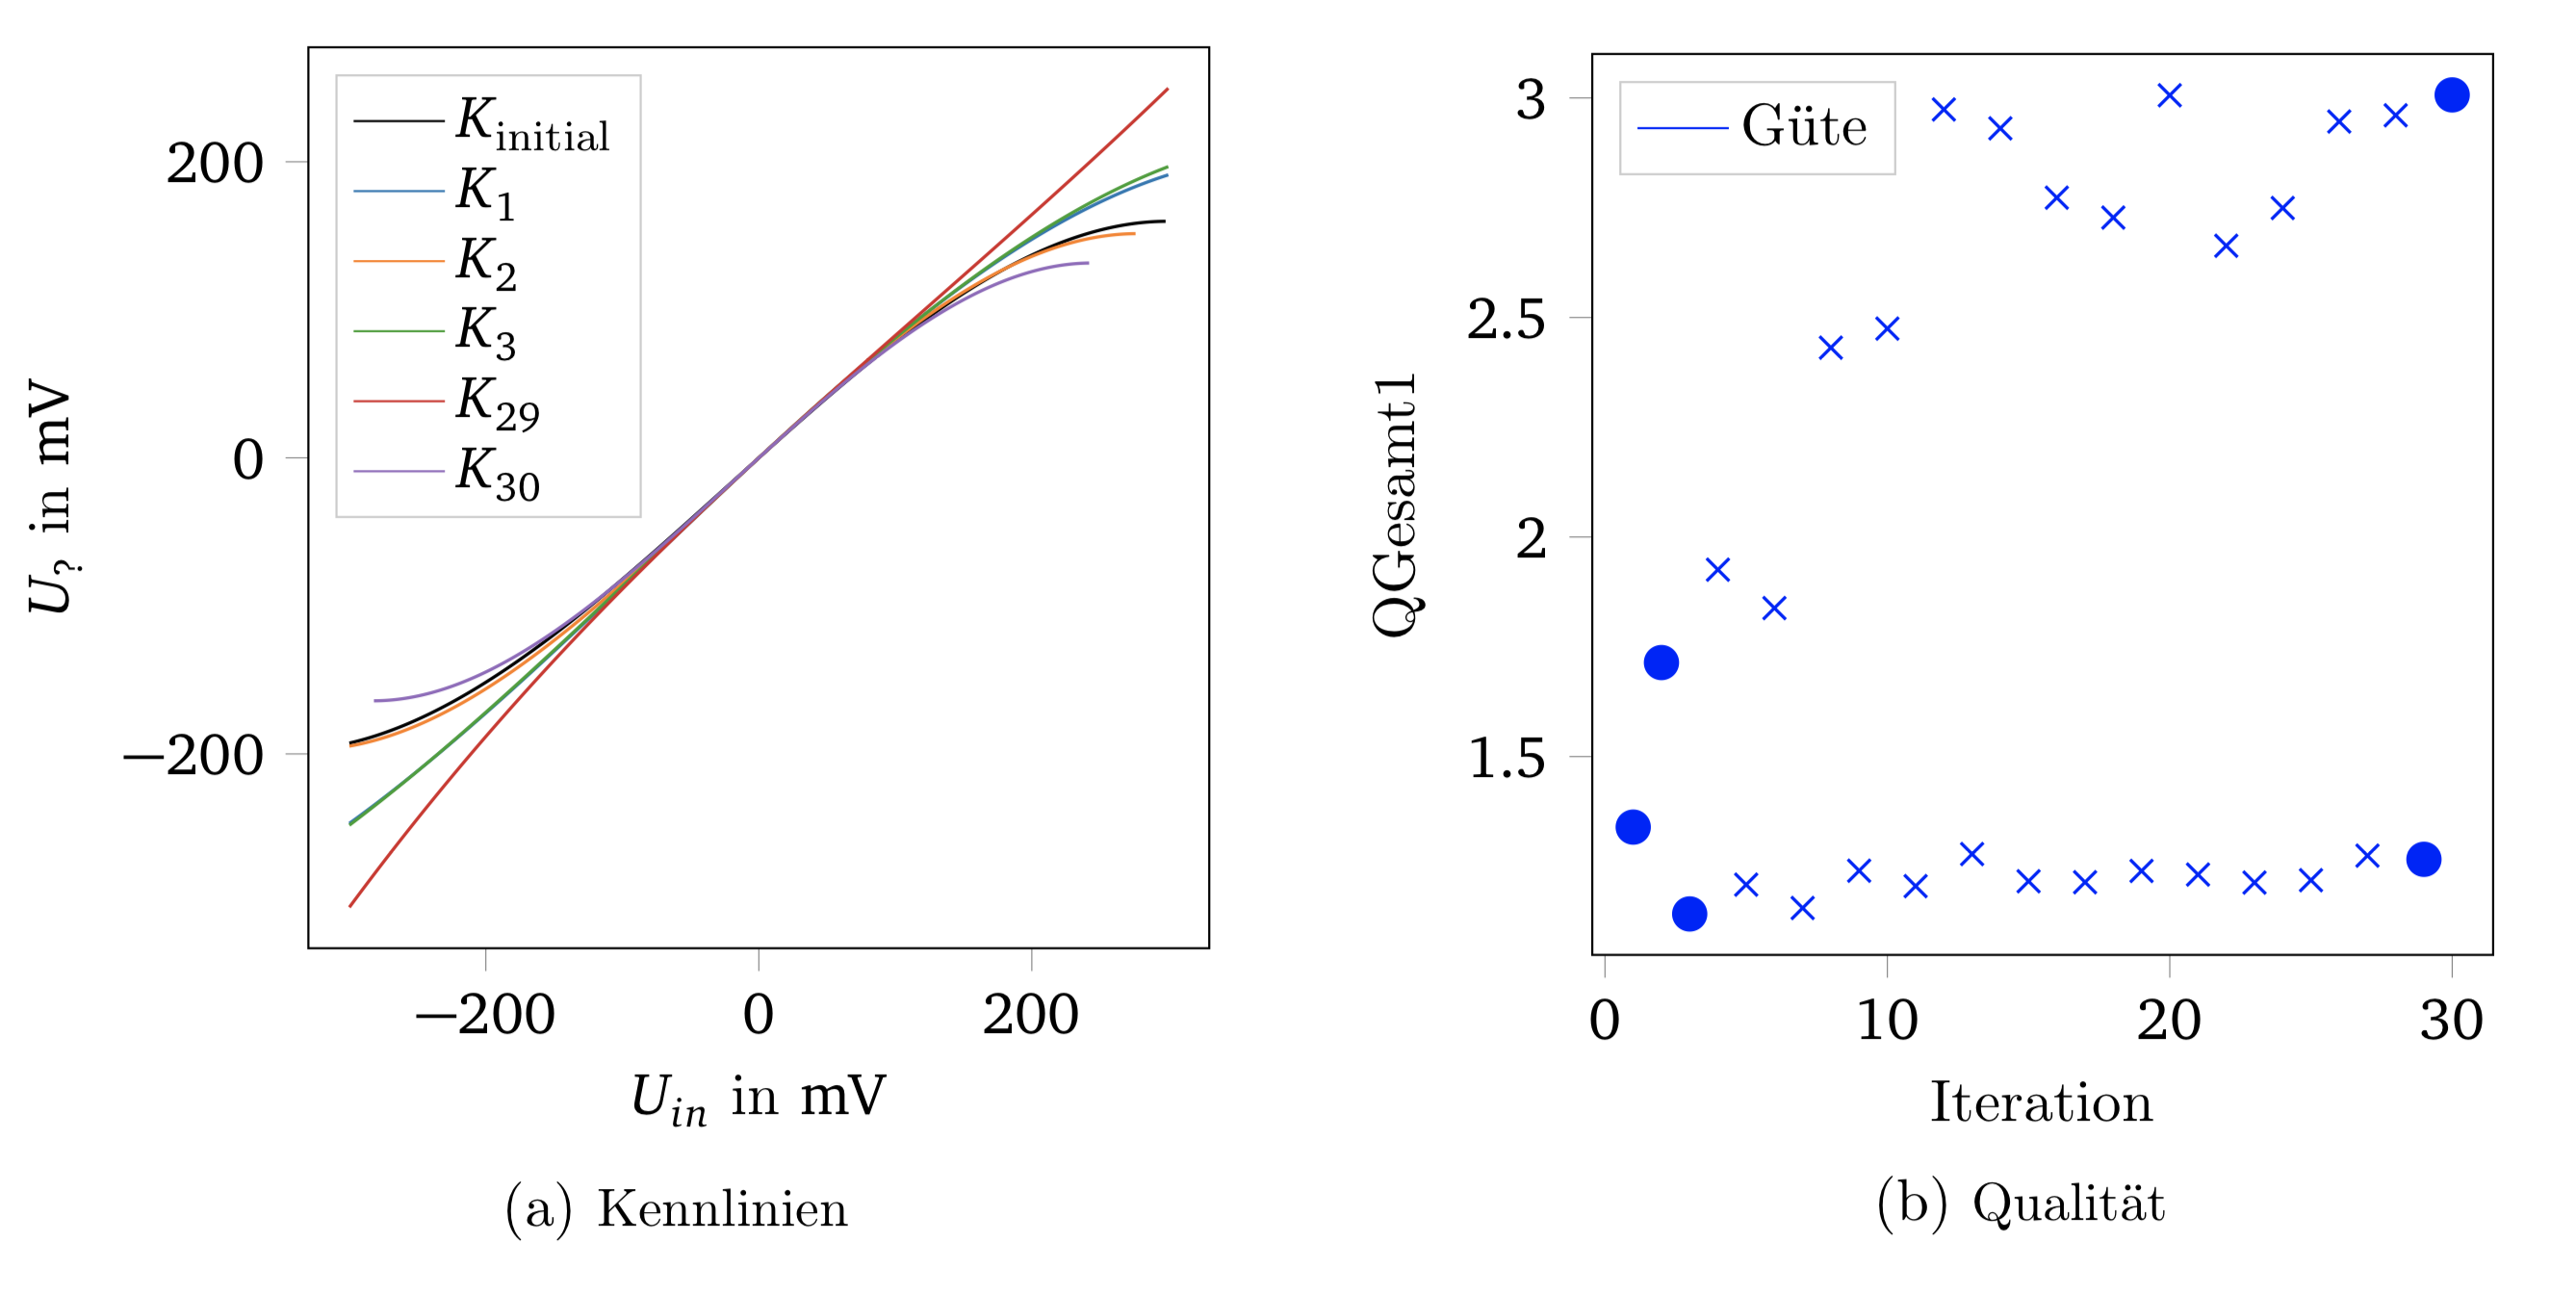
\includegraphics[scale=0.25]{slides/adjust_a/30Iteration.png} 
		}  
	\end{picture}
\end{frame}
%\begin{frame}
%\frametitle{Grenzen der Kennlinie}
%\begin{picture}(10,7)
%		\put(0,-160){
%			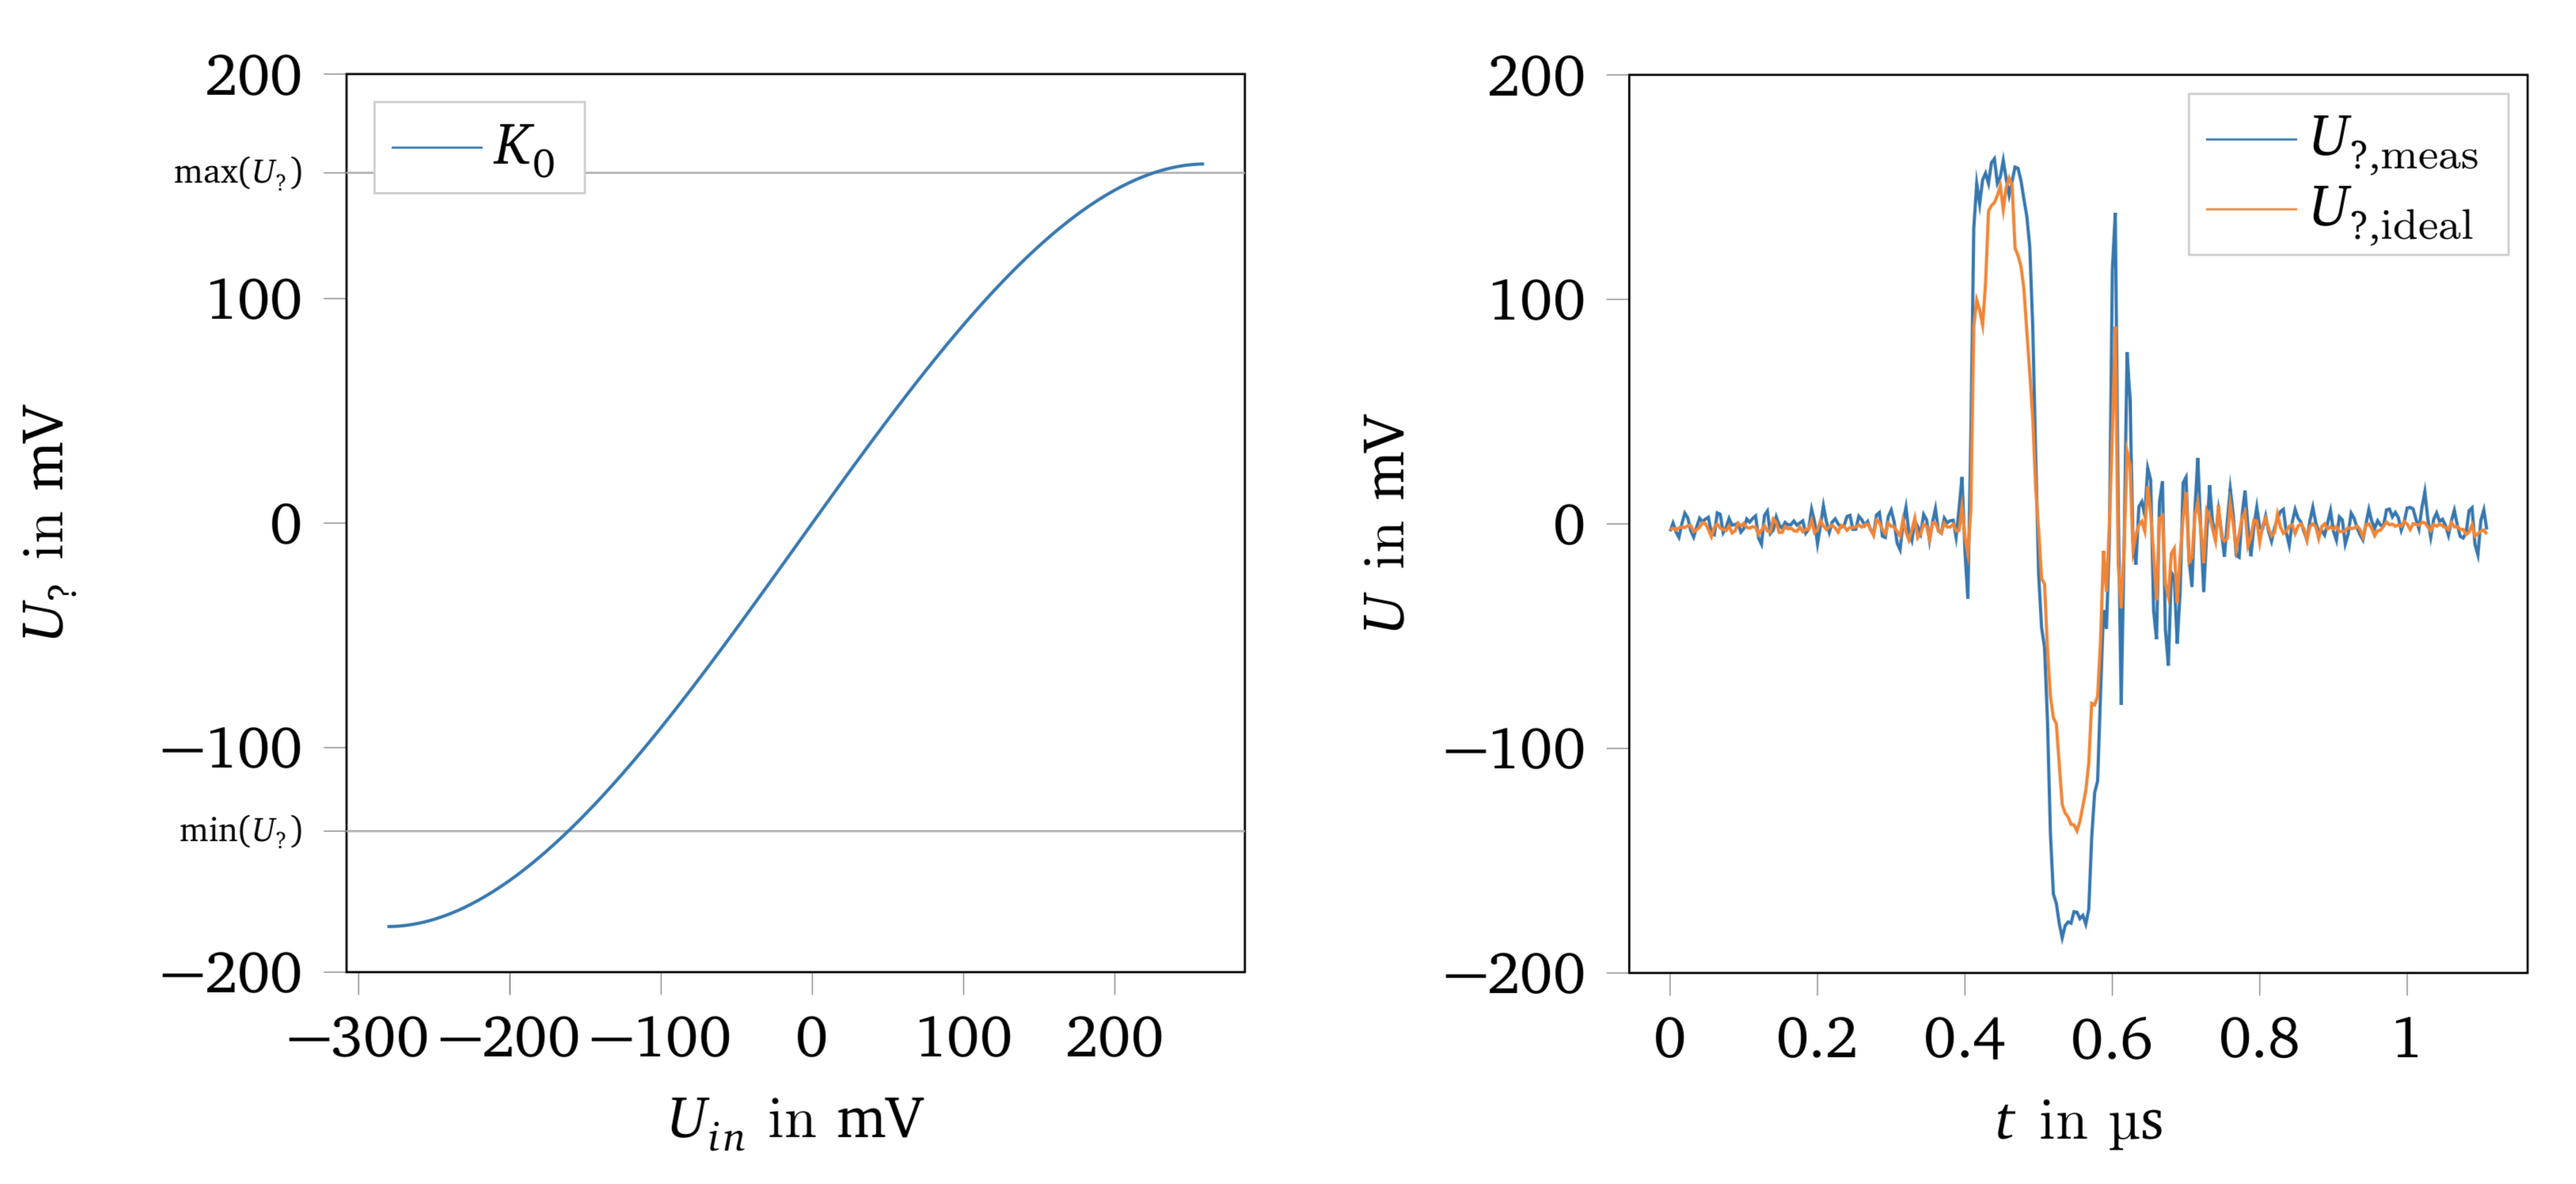
\includegraphics[scale=0.2]{slides/adjust_a/Grenzen_K.png} 
%		}  
%	\end{picture}
%\end{frame}
\begin{frame}
\frametitle{Grenzen der Kennlinie}
\begin{picture}(10,7)
		\put(-5,-150){
			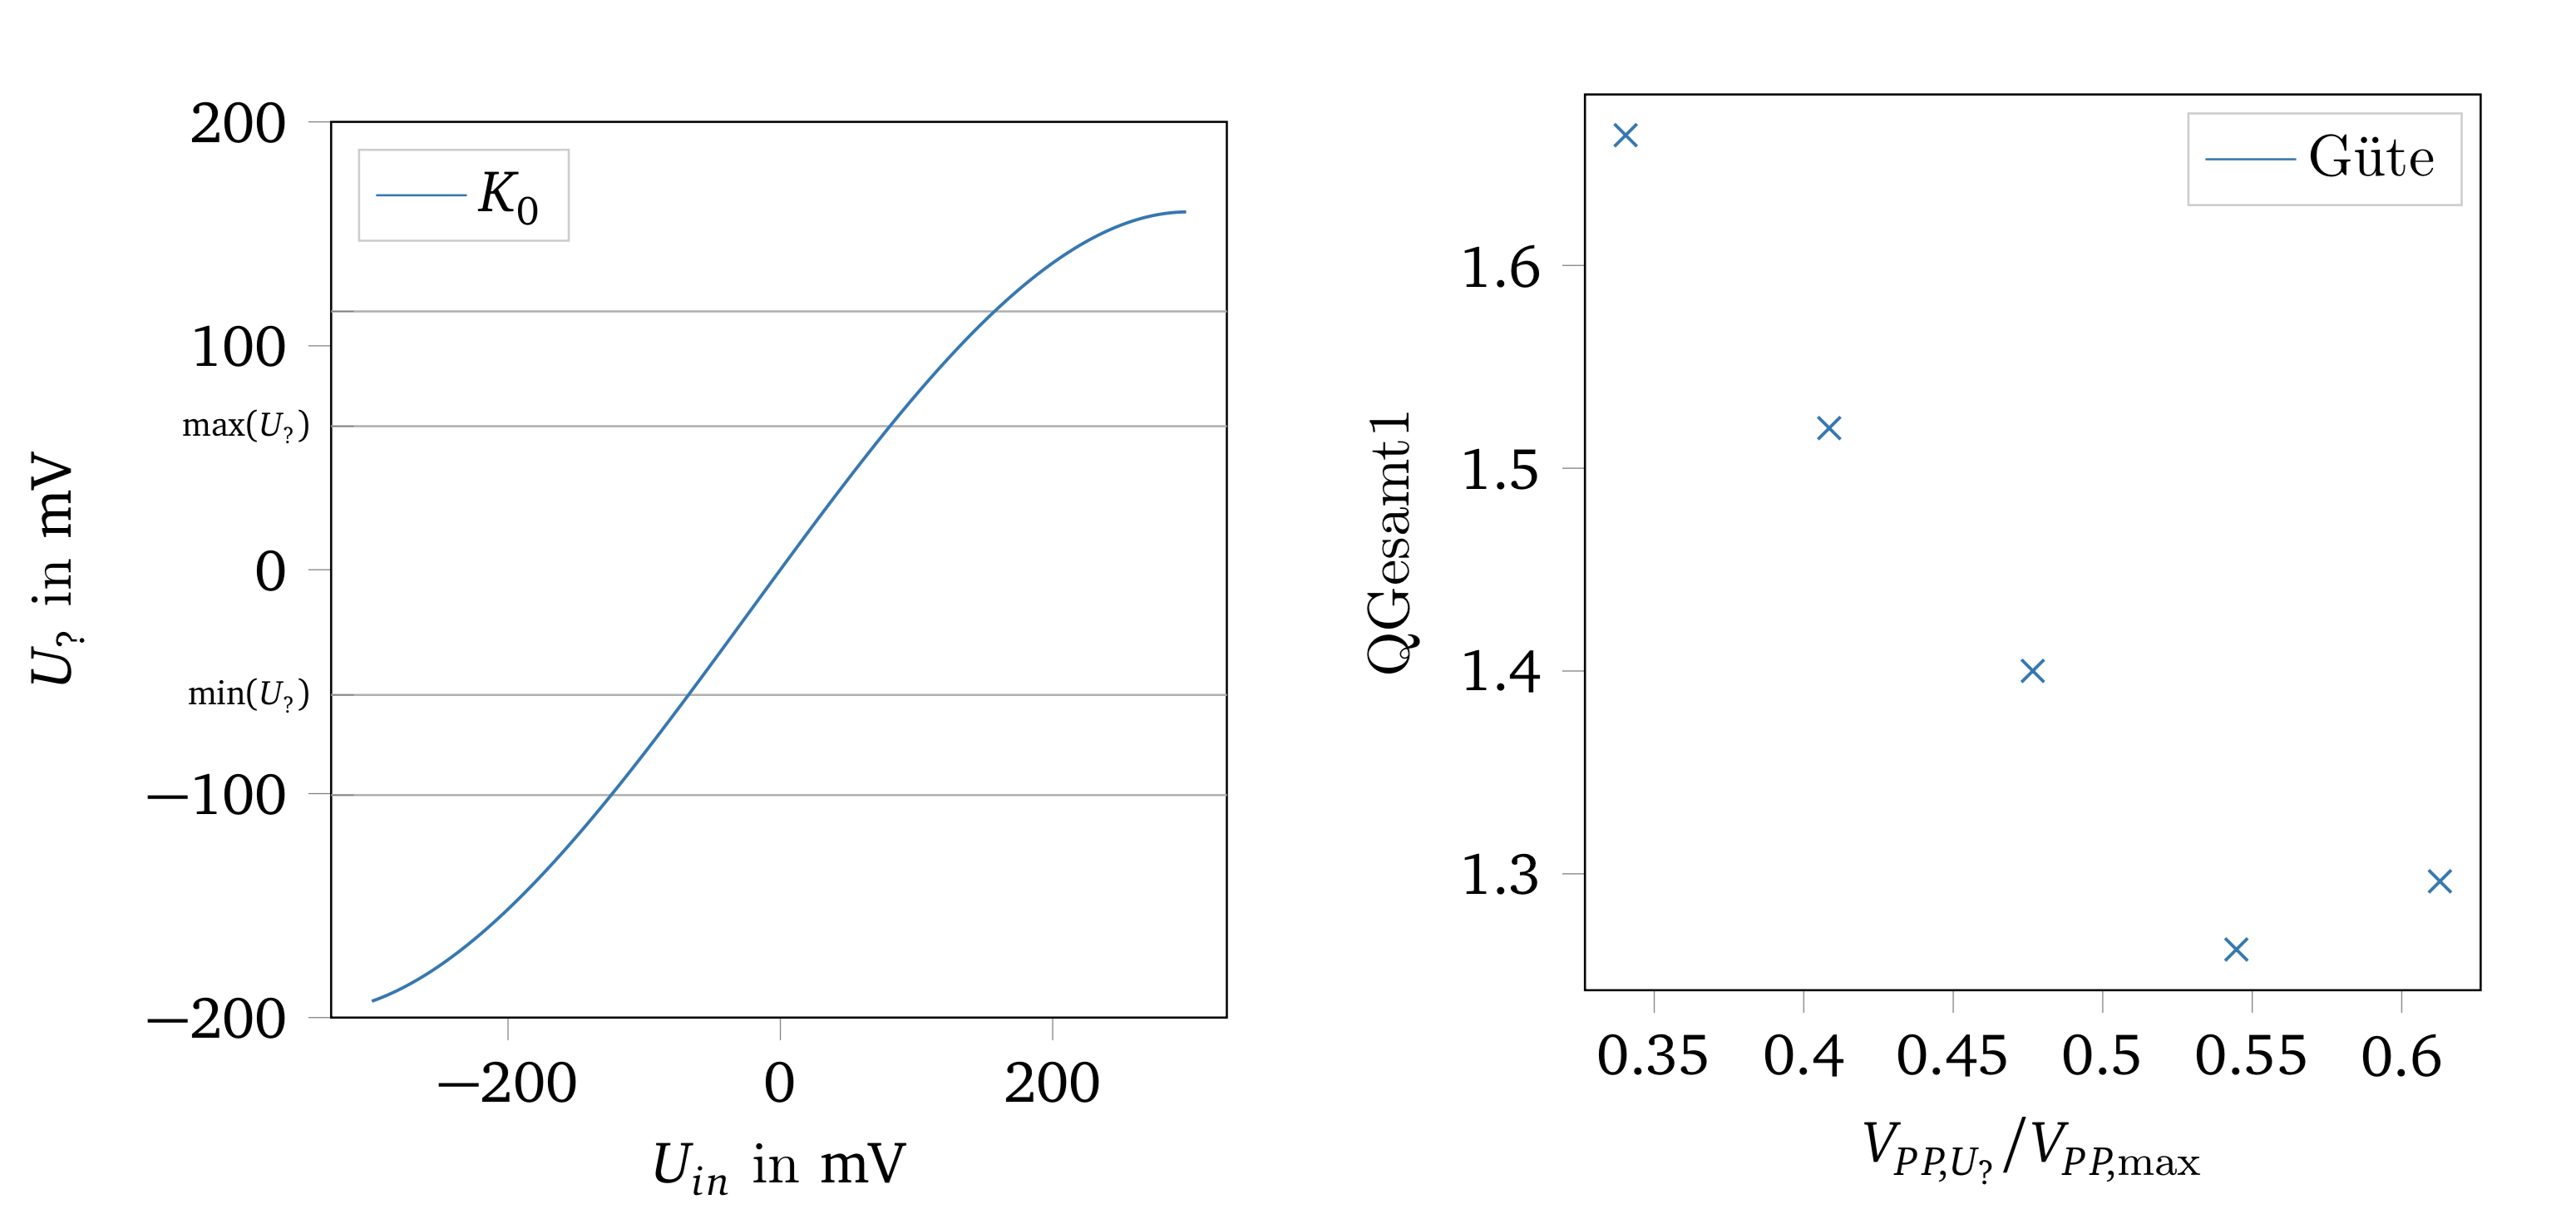
\includegraphics[scale=0.22]{slides/adjust_a/Grenzen_eval.png} 
		}  
	\end{picture}
\end{frame}
\begin{frame}
\frametitle{Zweiter Ansatz}
\begin{itemize}
	\item $K$ in einem kleineren Spannungsbereich anpassen
	\item Es wurden $66\%$ des maximal zulässigen Bereichs verwendet
\end{itemize}
\end{frame}

\begin{frame}
\frametitle{Zweiter Ansatz}
\begin{picture}(10,7)
		\put(-5,-150){
			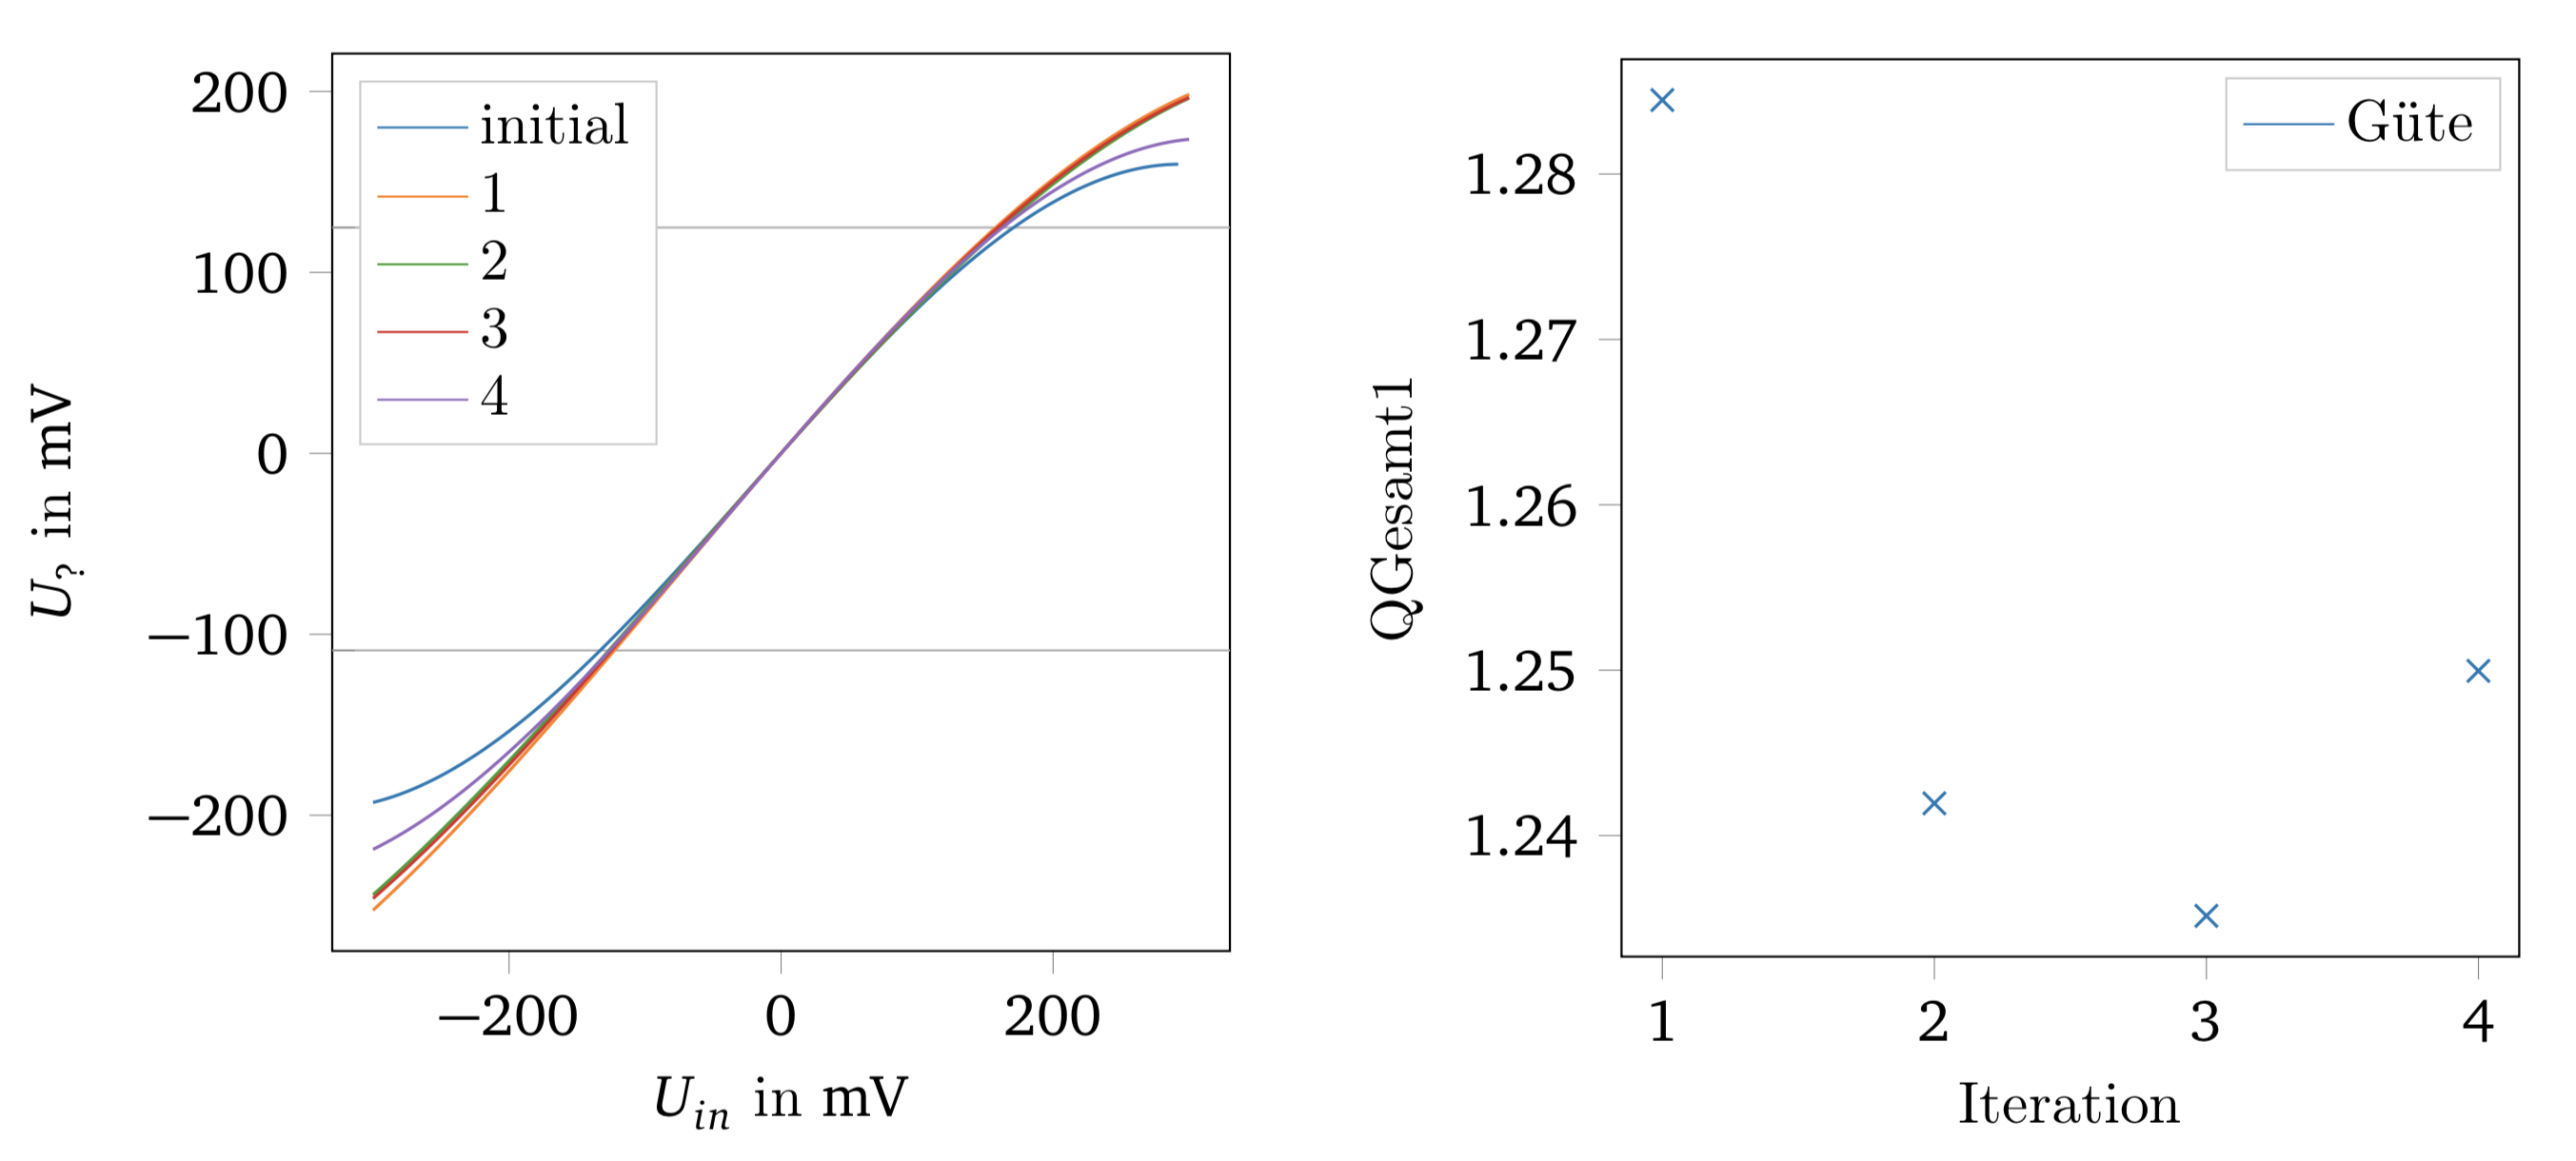
\includegraphics[scale=0.25]{slides/adjust_a/Zweiter_Versuch.png} 
		}  
	\end{picture}
\end{frame}

\begin{frame}
\frametitle{Offene Punkte}
\begin{itemize}
	\item Zweiter Ansatz mit mehr Iterationen Testen
	\item Die Grenzen für $K$ allgemein bestimmen
\end{itemize}
\end{frame}
